\subsection{Progettazione di Dettaglio e Codifica}

\subsubsection{Divisione oraria}
La seguente tabella rappresenta la distribuzione oraria dei ruoli per ogni componente del gruppo:
{
\rowcolors{2}{grigetto}{white}
\renewcommand{\arraystretch}{2}
\begin{longtable}[h!] { C{4cm} C{1cm} C{1cm} C{1cm} C{1cm} C{1cm} C{1cm} C{3cm}}
\caption{Tabella della divisione oraria della Progettazione di Dettaglio e Codifica}\\
\rowcolor{darkblue}

\textcolor{white}{\textbf{Membro del gruppo}} & 
\textcolor{white}{\textbf{RE}} & 
\textcolor{white}{\textbf{AM}} & 
\textcolor{white}{\textbf{AN}} & 
\textcolor{white}{\textbf{PT}} & 
\textcolor{white}{\textbf{PR}} & 
\textcolor{white}{\textbf{VE}} & 
\textcolor{white}{\textbf{Ore complessive}}\\
\endhead

\MC{}                     &  - & 10 & - & 13 &  16 &  11 &  50 \\
\LD{}                     &  6 &  - & - & 11 &  16 &  17 &  50 \\
\CE{}                     &  - &  5 & - & 14 &  17 &  14 &  50 \\
\SE{}                     &  - &  4 & - & 12 &  19 &  15 &  50 \\
\PF{}                     &  - &  8 & - &  9 &  20 &  13 &  50 \\
\DF{}                     & 10 &  - & - &  8 &  18 &  14 &  50 \\
\BR{}                     &  - &  3 & - & 13 &  20 &  14 &  50 \\
\AT{}                     & 10 &  - & - & 11 &  18 &  11 &  50 \\
\textbf{Ore totali ruolo} & 26 & 30 & - & 91 & 144 & 109 & 400 \\

\end{longtable}
}

La suddivisione di quante ore, ciascun componente del gruppo, ha svolto per ogni ruolo viene rappresentata nel seguente istogramma:
\begin{figure}[h!]
\centering
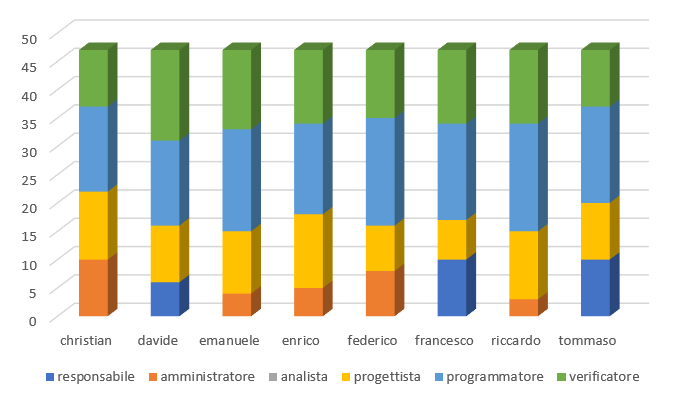
\includegraphics{Sezioni/Istogrammi/IstogrammaDiDettaglio.png}
\caption{Disposizione ore per ruolo di ciascun componente della fase di Progettazione di Dettaglio e Codifica}
\end{figure}

\clearpage

\subsubsection{Costo risultante}
La seguente tabella rappresenta, per ruolo, le ore totali investite e il corrispondente costo in euro:
{
\rowcolors{2}{grigetto}{white}
\renewcommand{\arraystretch}{2}
\begin{longtable}{ C{3cm} C{2cm} C{4cm}}
\caption{Tabella del costo risultante della Programmazione di Dettaglio e Codifica}\\
\rowcolor{darkblue}

\textcolor{white}{\textbf{Ruolo}} & 
\textcolor{white}{\textbf{Totale ore}} & 
\textcolor{white}{\textbf{Costo ruolo (in \euro{})}}\\	
\endhead
        
Responsabile    &  26 &  780 \\
Amministratore  &  30 &  600 \\
Analista        &   - &    - \\
Progettista     &  91 & 2002 \\
Programmatore   & 144 & 2160 \\
Verificatore    & 109 & 1635 \\
\textbf{Totale} & 400 & 7177 \\
		
\end{longtable}
}

La quantità di ore totali per ciascun ruolo viene rappresentata nel seguente areogramma:
\begin{figure}[h!]
	\centering	
	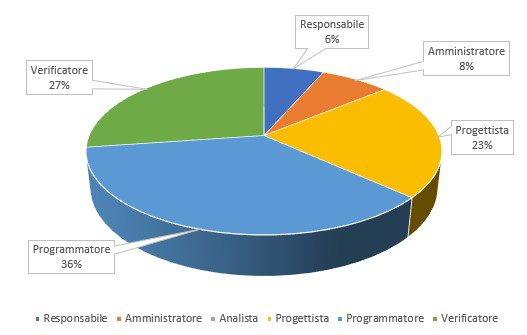
\includegraphics{Sezioni/Aerogrammi/AerogrammaDiDettaglio.png}
	\caption{Suddivisione ore per ruolo della fase di Progettazione di Dettaglio e Codifica}
\end{figure}